\documentclass[twoside]{book}

% Packages required by doxygen
\usepackage{fixltx2e}
\usepackage{calc}
\usepackage{doxygen}
\usepackage[export]{adjustbox} % also loads graphicx
\usepackage{graphicx}
\usepackage[utf8]{inputenc}
\usepackage{makeidx}
\usepackage{multicol}
\usepackage{multirow}
\PassOptionsToPackage{warn}{textcomp}
\usepackage{textcomp}
\usepackage[nointegrals]{wasysym}
\usepackage[table]{xcolor}

% Font selection
\usepackage[T1]{fontenc}
\usepackage[scaled=.90]{helvet}
\usepackage{courier}
\usepackage{amssymb}
\usepackage{sectsty}
\renewcommand{\familydefault}{\sfdefault}
\allsectionsfont{%
  \fontseries{bc}\selectfont%
  \color{darkgray}%
}
\renewcommand{\DoxyLabelFont}{%
  \fontseries{bc}\selectfont%
  \color{darkgray}%
}
\newcommand{\+}{\discretionary{\mbox{\scriptsize$\hookleftarrow$}}{}{}}

% Page & text layout
\usepackage{geometry}
\geometry{%
  a4paper,%
  top=2.5cm,%
  bottom=2.5cm,%
  left=2.5cm,%
  right=2.5cm%
}
\tolerance=750
\hfuzz=15pt
\hbadness=750
\setlength{\emergencystretch}{15pt}
\setlength{\parindent}{0cm}
\setlength{\parskip}{3ex plus 2ex minus 2ex}
\makeatletter
\renewcommand{\paragraph}{%
  \@startsection{paragraph}{4}{0ex}{-1.0ex}{1.0ex}{%
    \normalfont\normalsize\bfseries\SS@parafont%
  }%
}
\renewcommand{\subparagraph}{%
  \@startsection{subparagraph}{5}{0ex}{-1.0ex}{1.0ex}{%
    \normalfont\normalsize\bfseries\SS@subparafont%
  }%
}
\makeatother

% Headers & footers
\usepackage{fancyhdr}
\pagestyle{fancyplain}
\fancyhead[LE]{\fancyplain{}{\bfseries\thepage}}
\fancyhead[CE]{\fancyplain{}{}}
\fancyhead[RE]{\fancyplain{}{\bfseries\leftmark}}
\fancyhead[LO]{\fancyplain{}{\bfseries\rightmark}}
\fancyhead[CO]{\fancyplain{}{}}
\fancyhead[RO]{\fancyplain{}{\bfseries\thepage}}
\fancyfoot[LE]{\fancyplain{}{}}
\fancyfoot[CE]{\fancyplain{}{}}
\fancyfoot[RE]{\fancyplain{}{\bfseries\scriptsize Generated by Doxygen }}
\fancyfoot[LO]{\fancyplain{}{\bfseries\scriptsize Generated by Doxygen }}
\fancyfoot[CO]{\fancyplain{}{}}
\fancyfoot[RO]{\fancyplain{}{}}
\renewcommand{\footrulewidth}{0.4pt}
\renewcommand{\chaptermark}[1]{%
  \markboth{#1}{}%
}
\renewcommand{\sectionmark}[1]{%
  \markright{\thesection\ #1}%
}

% Indices & bibliography
\usepackage{natbib}
\usepackage[titles]{tocloft}
\setcounter{tocdepth}{3}
\setcounter{secnumdepth}{5}
\makeindex

% Hyperlinks (required, but should be loaded last)
\usepackage{ifpdf}
\ifpdf
  \usepackage[pdftex,pagebackref=true]{hyperref}
\else
  \usepackage[ps2pdf,pagebackref=true]{hyperref}
\fi
\hypersetup{%
  colorlinks=true,%
  linkcolor=blue,%
  citecolor=blue,%
  unicode%
}

% Custom commands
\newcommand{\clearemptydoublepage}{%
  \newpage{\pagestyle{empty}\cleardoublepage}%
}

\usepackage{caption}
\captionsetup{labelsep=space,justification=centering,font={bf},singlelinecheck=off,skip=4pt,position=top}

%===== C O N T E N T S =====

\begin{document}

% Titlepage & ToC
\hypersetup{pageanchor=false,
             bookmarksnumbered=true,
             pdfencoding=unicode
            }
\pagenumbering{alph}
\begin{titlepage}
\vspace*{7cm}
\begin{center}%
{\Large @C\+M\+A\+K\+E\+\_\+\+P\+R\+O\+J\+E\+C\+T\+\_\+\+N\+A\+ME@ }\\
\vspace*{1cm}
{\large Generated by Doxygen 1.8.14}\\
\end{center}
\end{titlepage}
\clearemptydoublepage
\pagenumbering{roman}
\tableofcontents
\clearemptydoublepage
\pagenumbering{arabic}
\hypersetup{pageanchor=true}

%--- Begin generated contents ---
\chapter{leistungsnachweis-\/firststeptoworlddomination}
\label{md__r_e_a_d_m_e}
\Hypertarget{md__r_e_a_d_m_e}
leistungsnachweis-\/firststeptoworlddomination created by Git\+Hub Classroom

Implementieren eines einfachen Q-\/\+Learning Algorithmus, der aus Interaktion mit einer Umgebung lernt.

Im ersten Schritt implementieren wir ein diskretes deterministisches Modell in einer statischen Umgebung. Das Modell soll dann in einem zweiten Schritt auf eine stochastische Umgebung erweitert werden und, falls der Umfang des Projekts das zu lässt, in einem weiteren Schritt auf eine dynamische Umgebung angepasst werden. 
\chapter{Hierarchical Index}
\section{Class Hierarchy}
This inheritance list is sorted roughly, but not completely, alphabetically\+:\begin{DoxyCompactList}
\item \contentsline{section}{Agent}{\pageref{class_agent}}{}
\begin{DoxyCompactList}
\item \contentsline{section}{Value\+Agent}{\pageref{class_value_agent}}{}
\end{DoxyCompactList}
\item \contentsline{section}{Environment}{\pageref{class_environment}}{}
\item \contentsline{section}{Num2\+D\+Table}{\pageref{class_num2_d_table}}{}
\item \contentsline{section}{Policy}{\pageref{class_policy}}{}
\begin{DoxyCompactList}
\item \contentsline{section}{Soft\+Max\+Policy}{\pageref{class_soft_max_policy}}{}
\item \contentsline{section}{Threshold\+Policy}{\pageref{class_threshold_policy}}{}
\end{DoxyCompactList}
\item \contentsline{section}{Q\+Values}{\pageref{class_q_values}}{}
\item \contentsline{section}{Environment\+:\+:Response}{\pageref{class_environment_1_1_response}}{}
\item Test\begin{DoxyCompactList}
\item \contentsline{section}{Agent\+Test}{\pageref{struct_agent_test}}{}
\end{DoxyCompactList}
\end{DoxyCompactList}

\chapter{Class Index}
\section{Class List}
Here are the classes, structs, unions and interfaces with brief descriptions\+:\begin{DoxyCompactList}
\item\contentsline{section}{\mbox{\hyperlink{class_agent}{Agent}} }{\pageref{class_agent}}{}
\item\contentsline{section}{\mbox{\hyperlink{struct_agent_test}{Agent\+Test}} }{\pageref{struct_agent_test}}{}
\item\contentsline{section}{\mbox{\hyperlink{class_environment}{Environment}} }{\pageref{class_environment}}{}
\item\contentsline{section}{\mbox{\hyperlink{class_num2_d_table}{Num2\+D\+Table}} }{\pageref{class_num2_d_table}}{}
\item\contentsline{section}{\mbox{\hyperlink{class_policy}{Policy}} }{\pageref{class_policy}}{}
\item\contentsline{section}{\mbox{\hyperlink{class_q_values}{Q\+Values}} }{\pageref{class_q_values}}{}
\item\contentsline{section}{\mbox{\hyperlink{class_environment_1_1_response}{Environment\+::\+Response}} }{\pageref{class_environment_1_1_response}}{}
\item\contentsline{section}{\mbox{\hyperlink{class_soft_max_policy}{Soft\+Max\+Policy}} }{\pageref{class_soft_max_policy}}{}
\item\contentsline{section}{\mbox{\hyperlink{class_threshold_policy}{Threshold\+Policy}} }{\pageref{class_threshold_policy}}{}
\item\contentsline{section}{\mbox{\hyperlink{class_value_agent}{Value\+Agent}} }{\pageref{class_value_agent}}{}
\end{DoxyCompactList}

\chapter{Class Documentation}
\hypertarget{class_agent}{}\section{Agent Class Reference}
\label{class_agent}\index{Agent@{Agent}}
Inheritance diagram for Agent\+:\begin{figure}[H]
\begin{center}
\leavevmode
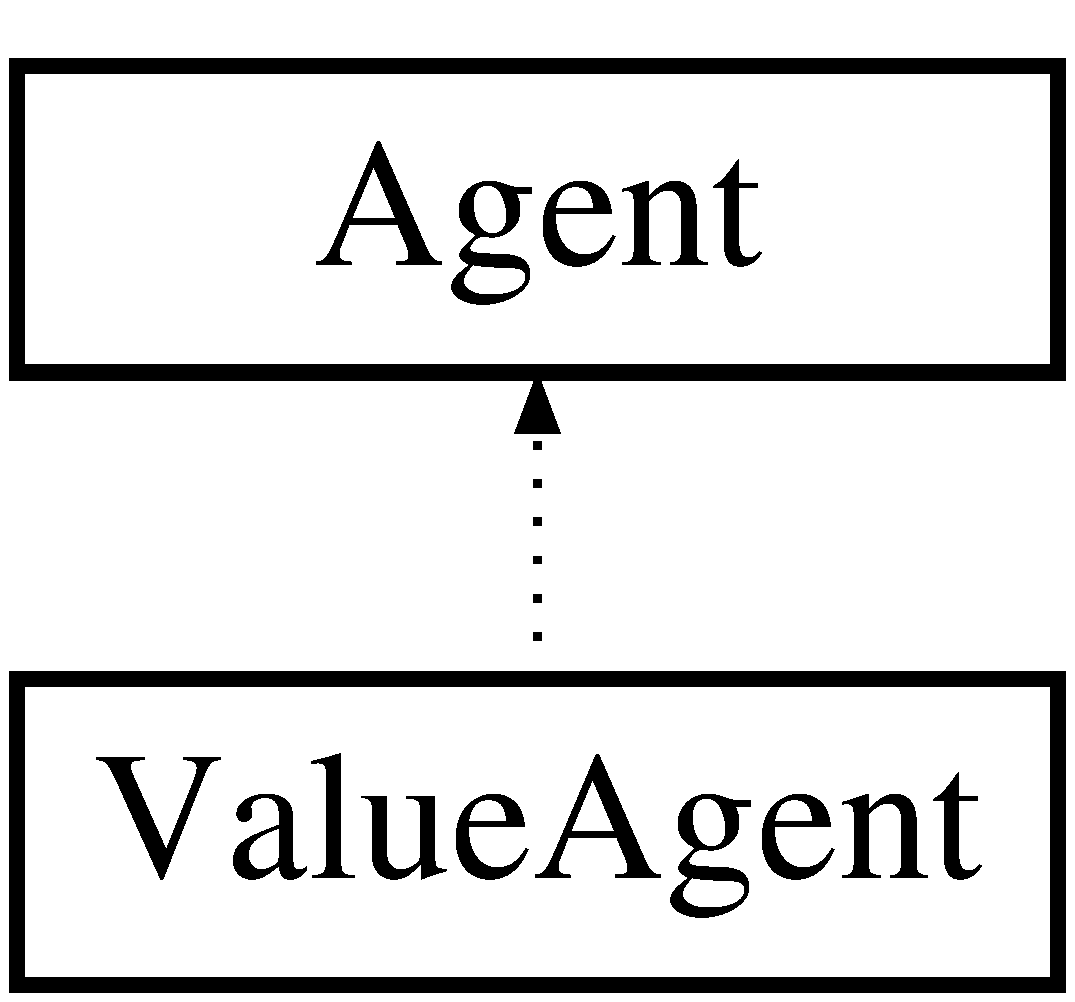
\includegraphics[height=2.000000cm]{class_agent}
\end{center}
\end{figure}
\subsection*{Public Member Functions}
\begin{DoxyCompactItemize}
\item 
\mbox{\hyperlink{class_agent_af202a4bd6845d8d2730e492f455785e3}{Agent}} (double learning\+Rate, double discount\+Rate, \mbox{\hyperlink{class_policy}{Policy}} $\ast$policy, \mbox{\hyperlink{class_environment}{Environment}} $\ast$env)
\item 
void \mbox{\hyperlink{class_agent_aa5716d6513268b2b5714a46341fb9006}{fit}} (int number\+Of\+Games)
\item 
\mbox{\Hypertarget{class_agent_a882df575e73539a3067087437a151b94}\label{class_agent_a882df575e73539a3067087437a151b94}} 
void {\bfseries debug} ()
\end{DoxyCompactItemize}
\subsection*{Friends}
\begin{DoxyCompactItemize}
\item 
\mbox{\Hypertarget{class_agent_ada6eaf56009c10f181cfc7b8e9957846}\label{class_agent_ada6eaf56009c10f181cfc7b8e9957846}} 
class {\bfseries Agent\+Test}
\item 
\mbox{\Hypertarget{class_agent_a7c64b6746f2b0b83e6ef1bbdfdd72245}\label{class_agent_a7c64b6746f2b0b83e6ef1bbdfdd72245}} 
class {\bfseries Policy}
\end{DoxyCompactItemize}


\subsection{Constructor \& Destructor Documentation}
\mbox{\Hypertarget{class_agent_af202a4bd6845d8d2730e492f455785e3}\label{class_agent_af202a4bd6845d8d2730e492f455785e3}} 
\index{Agent@{Agent}!Agent@{Agent}}
\index{Agent@{Agent}!Agent@{Agent}}
\subsubsection{\texorpdfstring{Agent()}{Agent()}}
{\footnotesize\ttfamily Agent\+::\+Agent (\begin{DoxyParamCaption}\item[{double}]{learning\+Rate,  }\item[{double}]{discount\+Rate,  }\item[{\mbox{\hyperlink{class_policy}{Policy}} $\ast$}]{policy,  }\item[{\mbox{\hyperlink{class_environment}{Environment}} $\ast$}]{env }\end{DoxyParamCaption})}

constructor 
\begin{DoxyParams}{Parameters}
{\em learning\+Rate} & alpha \\
\hline
{\em discount\+Rate} & gamma \\
\hline
{\em expl\+Rate} & probability of choosing a random action \\
\hline
{\em policy} & strategy for choosing next action \\
\hline
\end{DoxyParams}


\subsection{Member Function Documentation}
\mbox{\Hypertarget{class_agent_aa5716d6513268b2b5714a46341fb9006}\label{class_agent_aa5716d6513268b2b5714a46341fb9006}} 
\index{Agent@{Agent}!fit@{fit}}
\index{fit@{fit}!Agent@{Agent}}
\subsubsection{\texorpdfstring{fit()}{fit()}}
{\footnotesize\ttfamily void Agent\+::fit (\begin{DoxyParamCaption}\item[{int}]{number\+Of\+Games }\end{DoxyParamCaption})}

lets the agent learn from a given number of games 
\begin{DoxyParams}{Parameters}
{\em number\+Of\+Games} & number of games he is supposed to play \\
\hline
\end{DoxyParams}


The documentation for this class was generated from the following files\+:\begin{DoxyCompactItemize}
\item 
Agent.\+h\item 
Agent.\+cpp\end{DoxyCompactItemize}

\hypertarget{struct_agent_test}{}\section{Agent\+Test Struct Reference}
\label{struct_agent_test}\index{Agent\+Test@{Agent\+Test}}
Inheritance diagram for Agent\+Test\+:\begin{figure}[H]
\begin{center}
\leavevmode
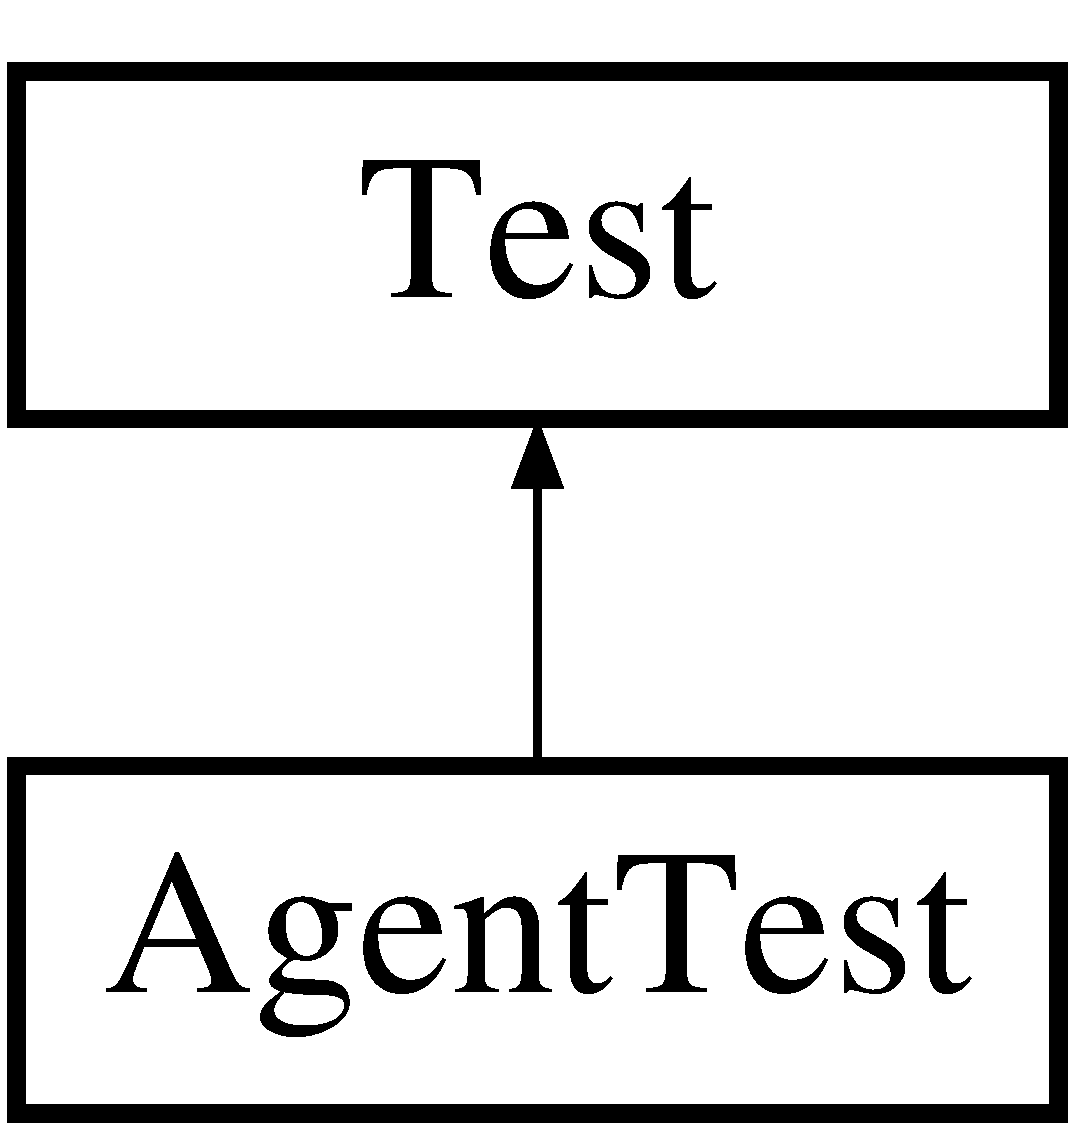
\includegraphics[height=2.000000cm]{struct_agent_test}
\end{center}
\end{figure}
\subsection*{Public Member Functions}
\begin{DoxyCompactItemize}
\item 
\mbox{\Hypertarget{struct_agent_test_a467ab33264562731ed09a47076816e29}\label{struct_agent_test_a467ab33264562731ed09a47076816e29}} 
void {\bfseries Set\+Up} ()
\item 
\mbox{\Hypertarget{struct_agent_test_adc6effea04ccb32c994552c46026102e}\label{struct_agent_test_adc6effea04ccb32c994552c46026102e}} 
void {\bfseries Tear\+Down} ()
\end{DoxyCompactItemize}
\subsection*{Public Attributes}
\begin{DoxyCompactItemize}
\item 
\mbox{\Hypertarget{struct_agent_test_a6faab5745a5cf6392bcf2326e5f87fc1}\label{struct_agent_test_a6faab5745a5cf6392bcf2326e5f87fc1}} 
\mbox{\hyperlink{class_agent}{Agent}} $\ast$ {\bfseries agent}
\item 
\mbox{\Hypertarget{struct_agent_test_a53b10928dc193dc3837e0c83539cdbf3}\label{struct_agent_test_a53b10928dc193dc3837e0c83539cdbf3}} 
\mbox{\hyperlink{class_threshold_policy}{Threshold\+Policy}} $\ast$ {\bfseries agent\+Policy}
\item 
\mbox{\Hypertarget{struct_agent_test_a29ce9e23c68d43632d7bcd53992f32cd}\label{struct_agent_test_a29ce9e23c68d43632d7bcd53992f32cd}} 
\mbox{\hyperlink{class_environment}{Environment}} $\ast$ {\bfseries environment}
\end{DoxyCompactItemize}


The documentation for this struct was generated from the following file\+:\begin{DoxyCompactItemize}
\item 
test\+Main.\+cpp\end{DoxyCompactItemize}

\hypertarget{class_environment}{}\section{Environment Class Reference}
\label{class_environment}\index{Environment@{Environment}}
\subsection*{Classes}
\begin{DoxyCompactItemize}
\item 
class \mbox{\hyperlink{class_environment_1_1_response}{Response}}
\end{DoxyCompactItemize}
\subsection*{Public Member Functions}
\begin{DoxyCompactItemize}
\item 
\mbox{\hyperlink{class_environment_a8b427c4448d8b7536666837521b9e83d}{Environment}} ()
\item 
\mbox{\hyperlink{class_environment_1_1_response}{Environment\+::\+Response}} $\ast$ \mbox{\hyperlink{class_environment_ab2531f3a79f25737da27ae5cac29ad05}{step}} (int action)
\item 
string \mbox{\hyperlink{class_environment_a7df8eab35d7ff6b7ce05eac019073ff1}{to\+String\+\_\+\+PG}} ()
\item 
string \mbox{\hyperlink{class_environment_aa542e4df56a2c6a2039fee9949052f0b}{to\+String\+\_\+\+RW}} ()
\item 
vector$<$ int $>$ $\ast$ \mbox{\hyperlink{class_environment_a98a9bfe041ae2fad721a96ee092fa45b}{get\+Actions}} ()
\item 
pair$<$ int, int $>$ $\ast$ \mbox{\hyperlink{class_environment_a7a7745adf6e9a0aec3b750e26e629f8b}{initial\+State}} ()
\item 
pair$<$ int, int $>$ $\ast$ \mbox{\hyperlink{class_environment_a93f31f5c387e9a470f49957f5a65aa31}{get\+State\+By\+Action}} (int action)
\item 
void \mbox{\hyperlink{class_environment_a9bf96c5e6b817be1595b24992cde8e82}{reset}} ()
\end{DoxyCompactItemize}
\subsection*{Friends}
\begin{DoxyCompactItemize}
\item 
\mbox{\Hypertarget{class_environment_ada6eaf56009c10f181cfc7b8e9957846}\label{class_environment_ada6eaf56009c10f181cfc7b8e9957846}} 
class {\bfseries Agent\+Test}
\end{DoxyCompactItemize}


\subsection{Constructor \& Destructor Documentation}
\mbox{\Hypertarget{class_environment_a8b427c4448d8b7536666837521b9e83d}\label{class_environment_a8b427c4448d8b7536666837521b9e83d}} 
\index{Environment@{Environment}!Environment@{Environment}}
\index{Environment@{Environment}!Environment@{Environment}}
\subsubsection{\texorpdfstring{Environment()}{Environment()}}
{\footnotesize\ttfamily Environment\+::\+Environment (\begin{DoxyParamCaption}{ }\end{DoxyParamCaption})\hspace{0.3cm}{\ttfamily [inline]}}

the game is stored here as a replay

actions taken by the agent are stored here

current play ground

possible rewards are saved here

the agents current position

the playgrouds shape \{rows,columns\}

\subsection{Member Function Documentation}
\mbox{\Hypertarget{class_environment_a98a9bfe041ae2fad721a96ee092fa45b}\label{class_environment_a98a9bfe041ae2fad721a96ee092fa45b}} 
\index{Environment@{Environment}!get\+Actions@{get\+Actions}}
\index{get\+Actions@{get\+Actions}!Environment@{Environment}}
\subsubsection{\texorpdfstring{get\+Actions()}{getActions()}}
{\footnotesize\ttfamily vector$<$ int $>$ $\ast$ Environment\+::get\+Actions (\begin{DoxyParamCaption}{ }\end{DoxyParamCaption})}

gives all possible actions from current state \begin{DoxyReturn}{Returns}
possible actions 
\end{DoxyReturn}
\mbox{\Hypertarget{class_environment_a93f31f5c387e9a470f49957f5a65aa31}\label{class_environment_a93f31f5c387e9a470f49957f5a65aa31}} 
\index{Environment@{Environment}!get\+State\+By\+Action@{get\+State\+By\+Action}}
\index{get\+State\+By\+Action@{get\+State\+By\+Action}!Environment@{Environment}}
\subsubsection{\texorpdfstring{get\+State\+By\+Action()}{getStateByAction()}}
{\footnotesize\ttfamily pair$<$ int, int $>$ $\ast$ Environment\+::get\+State\+By\+Action (\begin{DoxyParamCaption}\item[{int}]{action }\end{DoxyParamCaption})}

gives back the state corresponding to the result of an action taken from the current agent state 
\begin{DoxyParams}{Parameters}
{\em action} & to be taken \\
\hline
\end{DoxyParams}
\begin{DoxyReturn}{Returns}
the state of given action 
\end{DoxyReturn}
\mbox{\Hypertarget{class_environment_a7a7745adf6e9a0aec3b750e26e629f8b}\label{class_environment_a7a7745adf6e9a0aec3b750e26e629f8b}} 
\index{Environment@{Environment}!initial\+State@{initial\+State}}
\index{initial\+State@{initial\+State}!Environment@{Environment}}
\subsubsection{\texorpdfstring{initial\+State()}{initialState()}}
{\footnotesize\ttfamily pair$<$ int, int $>$ $\ast$ Environment\+::initial\+State (\begin{DoxyParamCaption}{ }\end{DoxyParamCaption})}

gives the initial state of the agent in the environment \begin{DoxyReturn}{Returns}
the initial state 
\end{DoxyReturn}
\mbox{\Hypertarget{class_environment_a9bf96c5e6b817be1595b24992cde8e82}\label{class_environment_a9bf96c5e6b817be1595b24992cde8e82}} 
\index{Environment@{Environment}!reset@{reset}}
\index{reset@{reset}!Environment@{Environment}}
\subsubsection{\texorpdfstring{reset()}{reset()}}
{\footnotesize\ttfamily void Environment\+::reset (\begin{DoxyParamCaption}{ }\end{DoxyParamCaption})}

resets the game \mbox{\Hypertarget{class_environment_ab2531f3a79f25737da27ae5cac29ad05}\label{class_environment_ab2531f3a79f25737da27ae5cac29ad05}} 
\index{Environment@{Environment}!step@{step}}
\index{step@{step}!Environment@{Environment}}
\subsubsection{\texorpdfstring{step()}{step()}}
{\footnotesize\ttfamily \mbox{\hyperlink{class_environment_1_1_response}{Environment\+::\+Response}} $\ast$ Environment\+::step (\begin{DoxyParamCaption}\item[{int}]{action }\end{DoxyParamCaption})}

takes a step in a certain direction  action\+: chosen action by the agent \begin{DoxyReturn}{Returns}
\mbox{\hyperlink{class_environment_1_1_response}{Response}} (state, options, reward, finished) 
\end{DoxyReturn}
\mbox{\Hypertarget{class_environment_a7df8eab35d7ff6b7ce05eac019073ff1}\label{class_environment_a7df8eab35d7ff6b7ce05eac019073ff1}} 
\index{Environment@{Environment}!to\+String\+\_\+\+PG@{to\+String\+\_\+\+PG}}
\index{to\+String\+\_\+\+PG@{to\+String\+\_\+\+PG}!Environment@{Environment}}
\subsubsection{\texorpdfstring{to\+String\+\_\+\+P\+G()}{toString\_PG()}}
{\footnotesize\ttfamily string Environment\+::to\+String\+\_\+\+PG (\begin{DoxyParamCaption}{ }\end{DoxyParamCaption})\hspace{0.3cm}{\ttfamily [inline]}}

generates a formated string of numerical values of the play ground \begin{DoxyReturn}{Returns}
plazground as string 
\end{DoxyReturn}
\mbox{\Hypertarget{class_environment_aa542e4df56a2c6a2039fee9949052f0b}\label{class_environment_aa542e4df56a2c6a2039fee9949052f0b}} 
\index{Environment@{Environment}!to\+String\+\_\+\+RW@{to\+String\+\_\+\+RW}}
\index{to\+String\+\_\+\+RW@{to\+String\+\_\+\+RW}!Environment@{Environment}}
\subsubsection{\texorpdfstring{to\+String\+\_\+\+R\+W()}{toString\_RW()}}
{\footnotesize\ttfamily string Environment\+::to\+String\+\_\+\+RW (\begin{DoxyParamCaption}{ }\end{DoxyParamCaption})\hspace{0.3cm}{\ttfamily [inline]}}

generates a formated string of numerical values of the reward map \begin{DoxyReturn}{Returns}
rewards as string 
\end{DoxyReturn}


The documentation for this class was generated from the following files\+:\begin{DoxyCompactItemize}
\item 
Environment.\+h\item 
Environment.\+cpp\end{DoxyCompactItemize}

\hypertarget{class_num2_d_table}{}\section{Num2\+D\+Table Class Reference}
\label{class_num2_d_table}\index{Num2\+D\+Table@{Num2\+D\+Table}}
\subsection*{Public Member Functions}
\begin{DoxyCompactItemize}
\item 
\mbox{\hyperlink{class_num2_d_table_ae2dd3716bfdb8a21dffde4c4a406f67a}{Num2\+D\+Table}} (pair$<$ int, int $>$ size)
\item 
\mbox{\hyperlink{class_num2_d_table_a43fbd24e26b1867ddd88a7b3d71c5d82}{Num2\+D\+Table}} (pair$<$ int, int $>$ size, vector$<$ double $>$ values)
\item 
\mbox{\hyperlink{class_num2_d_table_a059c6372eacdfc2d1e046190db443363}{Num2\+D\+Table}} ()=default
\item 
double \mbox{\hyperlink{class_num2_d_table_ac87a39a241ca9a1fa4e87ec6414761b7}{operator\mbox{[}$\,$\mbox{]}}} (const pair$<$ int, int $>$ index)
\item 
bool \mbox{\hyperlink{class_num2_d_table_a037b9168eac3a5d9f806fac1fd0e2a36}{operator==}} (const \mbox{\hyperlink{class_num2_d_table}{Num2\+D\+Table}} \&rhs) const
\item 
void \mbox{\hyperlink{class_num2_d_table_a218340f919c8382a00a11cf31abbff3e}{set\+Q\+Value}} (pair$<$ int, int $>$ index, double value)
\item 
bool \mbox{\hyperlink{class_num2_d_table_a97c0b41ef1b5a47fcc9fc9889453ec59}{key\+Exists}} (pair$<$ int, int $>$ index\+Pair)
\item 
string \mbox{\hyperlink{class_num2_d_table_a09def4905eca445abdccdb76224dcc85}{to\+String}} ()
\end{DoxyCompactItemize}
\subsection*{Public Attributes}
\begin{DoxyCompactItemize}
\item 
pair$<$ int, int $>$ \mbox{\hyperlink{class_num2_d_table_a4276fb2f2884e18421c165a22cdf23dc}{shape}}
\end{DoxyCompactItemize}


\subsection{Constructor \& Destructor Documentation}
\mbox{\Hypertarget{class_num2_d_table_ae2dd3716bfdb8a21dffde4c4a406f67a}\label{class_num2_d_table_ae2dd3716bfdb8a21dffde4c4a406f67a}} 
\index{Num2\+D\+Table@{Num2\+D\+Table}!Num2\+D\+Table@{Num2\+D\+Table}}
\index{Num2\+D\+Table@{Num2\+D\+Table}!Num2\+D\+Table@{Num2\+D\+Table}}
\subsubsection{\texorpdfstring{Num2\+D\+Table()}{Num2DTable()}\hspace{0.1cm}{\footnotesize\ttfamily [1/3]}}
{\footnotesize\ttfamily Num2\+D\+Table\+::\+Num2\+D\+Table (\begin{DoxyParamCaption}\item[{pair$<$ int, int $>$}]{size }\end{DoxyParamCaption})\hspace{0.3cm}{\ttfamily [inline]}, {\ttfamily [explicit]}}

constructor initializing table with a given size 
\begin{DoxyParams}{Parameters}
{\em size} & \\
\hline
\end{DoxyParams}
\mbox{\Hypertarget{class_num2_d_table_a43fbd24e26b1867ddd88a7b3d71c5d82}\label{class_num2_d_table_a43fbd24e26b1867ddd88a7b3d71c5d82}} 
\index{Num2\+D\+Table@{Num2\+D\+Table}!Num2\+D\+Table@{Num2\+D\+Table}}
\index{Num2\+D\+Table@{Num2\+D\+Table}!Num2\+D\+Table@{Num2\+D\+Table}}
\subsubsection{\texorpdfstring{Num2\+D\+Table()}{Num2DTable()}\hspace{0.1cm}{\footnotesize\ttfamily [2/3]}}
{\footnotesize\ttfamily Num2\+D\+Table\+::\+Num2\+D\+Table (\begin{DoxyParamCaption}\item[{pair$<$ int, int $>$}]{size,  }\item[{vector$<$ double $>$}]{values }\end{DoxyParamCaption})\hspace{0.3cm}{\ttfamily [inline]}}

constructor initializing table with a given size and values 
\begin{DoxyParams}{Parameters}
{\em size} & \\
\hline
{\em values} & \\
\hline
\end{DoxyParams}
\mbox{\Hypertarget{class_num2_d_table_a059c6372eacdfc2d1e046190db443363}\label{class_num2_d_table_a059c6372eacdfc2d1e046190db443363}} 
\index{Num2\+D\+Table@{Num2\+D\+Table}!Num2\+D\+Table@{Num2\+D\+Table}}
\index{Num2\+D\+Table@{Num2\+D\+Table}!Num2\+D\+Table@{Num2\+D\+Table}}
\subsubsection{\texorpdfstring{Num2\+D\+Table()}{Num2DTable()}\hspace{0.1cm}{\footnotesize\ttfamily [3/3]}}
{\footnotesize\ttfamily Num2\+D\+Table\+::\+Num2\+D\+Table (\begin{DoxyParamCaption}{ }\end{DoxyParamCaption})\hspace{0.3cm}{\ttfamily [default]}}

default constructor 

\subsection{Member Function Documentation}
\mbox{\Hypertarget{class_num2_d_table_a97c0b41ef1b5a47fcc9fc9889453ec59}\label{class_num2_d_table_a97c0b41ef1b5a47fcc9fc9889453ec59}} 
\index{Num2\+D\+Table@{Num2\+D\+Table}!key\+Exists@{key\+Exists}}
\index{key\+Exists@{key\+Exists}!Num2\+D\+Table@{Num2\+D\+Table}}
\subsubsection{\texorpdfstring{key\+Exists()}{keyExists()}}
{\footnotesize\ttfamily bool Num2\+D\+Table\+::key\+Exists (\begin{DoxyParamCaption}\item[{pair$<$ int, int $>$}]{index\+Pair }\end{DoxyParamCaption})\hspace{0.3cm}{\ttfamily [inline]}}

checks if the given index pair is within the table 
\begin{DoxyParams}{Parameters}
{\em index\+Pair} & \\
\hline
\end{DoxyParams}
\begin{DoxyReturn}{Returns}
true or false 
\end{DoxyReturn}
\mbox{\Hypertarget{class_num2_d_table_a037b9168eac3a5d9f806fac1fd0e2a36}\label{class_num2_d_table_a037b9168eac3a5d9f806fac1fd0e2a36}} 
\index{Num2\+D\+Table@{Num2\+D\+Table}!operator==@{operator==}}
\index{operator==@{operator==}!Num2\+D\+Table@{Num2\+D\+Table}}
\subsubsection{\texorpdfstring{operator==()}{operator==()}}
{\footnotesize\ttfamily bool Num2\+D\+Table\+::operator== (\begin{DoxyParamCaption}\item[{const \mbox{\hyperlink{class_num2_d_table}{Num2\+D\+Table}} \&}]{rhs }\end{DoxyParamCaption}) const\hspace{0.3cm}{\ttfamily [inline]}}

defines operater == for testing purposes 
\begin{DoxyParams}{Parameters}
{\em rhs} & \\
\hline
\end{DoxyParams}
\begin{DoxyReturn}{Returns}
true or false 
\end{DoxyReturn}
\mbox{\Hypertarget{class_num2_d_table_ac87a39a241ca9a1fa4e87ec6414761b7}\label{class_num2_d_table_ac87a39a241ca9a1fa4e87ec6414761b7}} 
\index{Num2\+D\+Table@{Num2\+D\+Table}!operator\mbox{[}\mbox{]}@{operator[]}}
\index{operator\mbox{[}\mbox{]}@{operator[]}!Num2\+D\+Table@{Num2\+D\+Table}}
\subsubsection{\texorpdfstring{operator[]()}{operator[]()}}
{\footnotesize\ttfamily double Num2\+D\+Table\+::operator\mbox{[}$\,$\mbox{]} (\begin{DoxyParamCaption}\item[{const pair$<$ int, int $>$}]{index }\end{DoxyParamCaption})\hspace{0.3cm}{\ttfamily [inline]}}

defines operator \mbox{[}\mbox{]} to be able to get values from vector with given pair indices 
\begin{DoxyParams}{Parameters}
{\em index} & pair \\
\hline
\end{DoxyParams}
\begin{DoxyReturn}{Returns}
wanted value 
\end{DoxyReturn}
\mbox{\Hypertarget{class_num2_d_table_a218340f919c8382a00a11cf31abbff3e}\label{class_num2_d_table_a218340f919c8382a00a11cf31abbff3e}} 
\index{Num2\+D\+Table@{Num2\+D\+Table}!set\+Q\+Value@{set\+Q\+Value}}
\index{set\+Q\+Value@{set\+Q\+Value}!Num2\+D\+Table@{Num2\+D\+Table}}
\subsubsection{\texorpdfstring{set\+Q\+Value()}{setQValue()}}
{\footnotesize\ttfamily void Num2\+D\+Table\+::set\+Q\+Value (\begin{DoxyParamCaption}\item[{pair$<$ int, int $>$}]{index,  }\item[{double}]{value }\end{DoxyParamCaption})\hspace{0.3cm}{\ttfamily [inline]}}

stores a given value into the value vector at given pair index 
\begin{DoxyParams}{Parameters}
{\em index} & pair \\
\hline
{\em value} & \\
\hline
\end{DoxyParams}
\mbox{\Hypertarget{class_num2_d_table_a09def4905eca445abdccdb76224dcc85}\label{class_num2_d_table_a09def4905eca445abdccdb76224dcc85}} 
\index{Num2\+D\+Table@{Num2\+D\+Table}!to\+String@{to\+String}}
\index{to\+String@{to\+String}!Num2\+D\+Table@{Num2\+D\+Table}}
\subsubsection{\texorpdfstring{to\+String()}{toString()}}
{\footnotesize\ttfamily string Num2\+D\+Table\+::to\+String (\begin{DoxyParamCaption}{ }\end{DoxyParamCaption})\hspace{0.3cm}{\ttfamily [inline]}}

\mbox{\hyperlink{class_num2_d_table}{Num2\+D\+Table}} as string \begin{DoxyReturn}{Returns}
\mbox{\hyperlink{class_num2_d_table}{Num2\+D\+Table}} as string 
\end{DoxyReturn}


\subsection{Member Data Documentation}
\mbox{\Hypertarget{class_num2_d_table_a4276fb2f2884e18421c165a22cdf23dc}\label{class_num2_d_table_a4276fb2f2884e18421c165a22cdf23dc}} 
\index{Num2\+D\+Table@{Num2\+D\+Table}!shape@{shape}}
\index{shape@{shape}!Num2\+D\+Table@{Num2\+D\+Table}}
\subsubsection{\texorpdfstring{shape}{shape}}
{\footnotesize\ttfamily pair$<$int,int$>$ Num2\+D\+Table\+::shape}

the shape$<$row, column$>$ 

The documentation for this class was generated from the following file\+:\begin{DoxyCompactItemize}
\item 
Num2\+D\+Table.\+h\end{DoxyCompactItemize}

\hypertarget{class_policy}{}\section{Policy Class Reference}
\label{class_policy}\index{Policy@{Policy}}
Inheritance diagram for Policy\+:\begin{figure}[H]
\begin{center}
\leavevmode
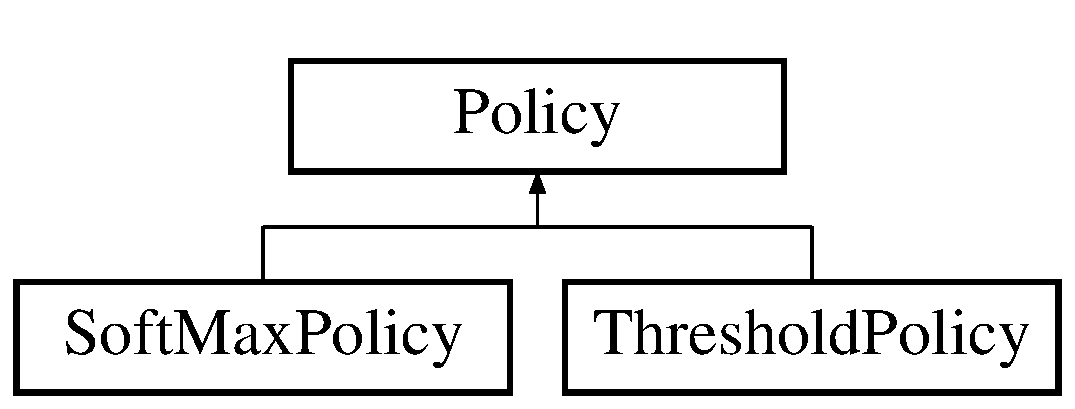
\includegraphics[height=2.000000cm]{class_policy}
\end{center}
\end{figure}
\subsection*{Public Member Functions}
\begin{DoxyCompactItemize}
\item 
virtual int \mbox{\hyperlink{class_policy_a7afb2eee3c77b96a58d992acb4e0e1a8}{choose\+Action}} (vector$<$ int $>$ possible\+Actions, vector$<$ double $>$ num\+Values)
\end{DoxyCompactItemize}


\subsection{Member Function Documentation}
\mbox{\Hypertarget{class_policy_a7afb2eee3c77b96a58d992acb4e0e1a8}\label{class_policy_a7afb2eee3c77b96a58d992acb4e0e1a8}} 
\index{Policy@{Policy}!choose\+Action@{choose\+Action}}
\index{choose\+Action@{choose\+Action}!Policy@{Policy}}
\subsubsection{\texorpdfstring{choose\+Action()}{chooseAction()}}
{\footnotesize\ttfamily virtual int Policy\+::choose\+Action (\begin{DoxyParamCaption}\item[{vector$<$ int $>$}]{possible\+Actions,  }\item[{vector$<$ double $>$}]{num\+Values }\end{DoxyParamCaption})\hspace{0.3cm}{\ttfamily [inline]}, {\ttfamily [virtual]}}

chooses the next action 
\begin{DoxyParams}{Parameters}
{\em possible\+Actions} & \\
\hline
{\em num\+Values} & \\
\hline
\end{DoxyParams}
\begin{DoxyReturn}{Returns}
next action 
\end{DoxyReturn}


Reimplemented in \mbox{\hyperlink{class_threshold_policy_a9f8e4051589b915971ffc647ba7fe623}{Threshold\+Policy}}, and \mbox{\hyperlink{class_soft_max_policy_a425d8bb5f2f504f2d7de8576f0e3f81f}{Soft\+Max\+Policy}}.



The documentation for this class was generated from the following file\+:\begin{DoxyCompactItemize}
\item 
Policy.\+h\end{DoxyCompactItemize}

\hypertarget{class_q_values}{}\section{Q\+Values Class Reference}
\label{class_q_values}\index{Q\+Values@{Q\+Values}}


The documentation for this class was generated from the following file\+:\begin{DoxyCompactItemize}
\item 
q\+Values.\+h\end{DoxyCompactItemize}

\hypertarget{class_environment_1_1_response}{}\section{Environment\+:\+:Response Class Reference}
\label{class_environment_1_1_response}\index{Environment\+::\+Response@{Environment\+::\+Response}}
\subsection*{Public Member Functions}
\begin{DoxyCompactItemize}
\item 
\mbox{\hyperlink{class_environment_1_1_response_a99c21b13f5806fd46bb656b52eddd6a5}{Response}} (pair$<$ int, int $>$ $\ast$\mbox{\hyperlink{class_environment_1_1_response_ab20f0a5064e6c7bec33600efce584489}{state}}, vector$<$ int $>$ \mbox{\hyperlink{class_environment_1_1_response_a201983545c18d0898382b7f073528ace}{options}}, double \mbox{\hyperlink{class_environment_1_1_response_a38f0083f3e1de4a30c2379de47625943}{reward}}, bool \mbox{\hyperlink{class_environment_1_1_response_a8becce546198aaec1e782cd38fbe1934}{finished}})
\item 
\mbox{\Hypertarget{class_environment_1_1_response_a7c8416b8a5ff7a7a4115f36effc31ab5}\label{class_environment_1_1_response_a7c8416b8a5ff7a7a4115f36effc31ab5}} 
string {\bfseries to\+String} ()
\end{DoxyCompactItemize}
\subsection*{Public Attributes}
\begin{DoxyCompactItemize}
\item 
pair$<$ int, int $>$ $\ast$ \mbox{\hyperlink{class_environment_1_1_response_ab20f0a5064e6c7bec33600efce584489}{state}}
\item 
vector$<$ int $>$ \mbox{\hyperlink{class_environment_1_1_response_a201983545c18d0898382b7f073528ace}{options}}
\item 
double \mbox{\hyperlink{class_environment_1_1_response_a38f0083f3e1de4a30c2379de47625943}{reward}}
\item 
bool \mbox{\hyperlink{class_environment_1_1_response_a8becce546198aaec1e782cd38fbe1934}{finished}} = false
\end{DoxyCompactItemize}


\subsection{Constructor \& Destructor Documentation}
\mbox{\Hypertarget{class_environment_1_1_response_a99c21b13f5806fd46bb656b52eddd6a5}\label{class_environment_1_1_response_a99c21b13f5806fd46bb656b52eddd6a5}} 
\index{Environment\+::\+Response@{Environment\+::\+Response}!Response@{Response}}
\index{Response@{Response}!Environment\+::\+Response@{Environment\+::\+Response}}
\subsubsection{\texorpdfstring{Response()}{Response()}}
{\footnotesize\ttfamily Environment\+::\+Response\+::\+Response (\begin{DoxyParamCaption}\item[{pair$<$ int, int $>$ $\ast$}]{state,  }\item[{vector$<$ int $>$}]{options,  }\item[{double}]{reward,  }\item[{bool}]{finished }\end{DoxyParamCaption})\hspace{0.3cm}{\ttfamily [inline]}}

constructor 
\begin{DoxyParams}{Parameters}
{\em state} & after the agent chose a step \\
\hline
{\em options} & of his new possible actions \\
\hline
{\em reward} & after moving a step \\
\hline
{\em finished} & whether the step has led to a game finish or not \\
\hline
\end{DoxyParams}


\subsection{Member Data Documentation}
\mbox{\Hypertarget{class_environment_1_1_response_a8becce546198aaec1e782cd38fbe1934}\label{class_environment_1_1_response_a8becce546198aaec1e782cd38fbe1934}} 
\index{Environment\+::\+Response@{Environment\+::\+Response}!finished@{finished}}
\index{finished@{finished}!Environment\+::\+Response@{Environment\+::\+Response}}
\subsubsection{\texorpdfstring{finished}{finished}}
{\footnotesize\ttfamily bool Environment\+::\+Response\+::finished = false}

indicates if game is over \mbox{\Hypertarget{class_environment_1_1_response_a201983545c18d0898382b7f073528ace}\label{class_environment_1_1_response_a201983545c18d0898382b7f073528ace}} 
\index{Environment\+::\+Response@{Environment\+::\+Response}!options@{options}}
\index{options@{options}!Environment\+::\+Response@{Environment\+::\+Response}}
\subsubsection{\texorpdfstring{options}{options}}
{\footnotesize\ttfamily vector$<$int$>$ Environment\+::\+Response\+::options}

vector of all possible actions \mbox{\Hypertarget{class_environment_1_1_response_a38f0083f3e1de4a30c2379de47625943}\label{class_environment_1_1_response_a38f0083f3e1de4a30c2379de47625943}} 
\index{Environment\+::\+Response@{Environment\+::\+Response}!reward@{reward}}
\index{reward@{reward}!Environment\+::\+Response@{Environment\+::\+Response}}
\subsubsection{\texorpdfstring{reward}{reward}}
{\footnotesize\ttfamily double Environment\+::\+Response\+::reward}

reward earned \mbox{\Hypertarget{class_environment_1_1_response_ab20f0a5064e6c7bec33600efce584489}\label{class_environment_1_1_response_ab20f0a5064e6c7bec33600efce584489}} 
\index{Environment\+::\+Response@{Environment\+::\+Response}!state@{state}}
\index{state@{state}!Environment\+::\+Response@{Environment\+::\+Response}}
\subsubsection{\texorpdfstring{state}{state}}
{\footnotesize\ttfamily pair$<$int, int$>$$\ast$ Environment\+::\+Response\+::state}

game state 

The documentation for this class was generated from the following file\+:\begin{DoxyCompactItemize}
\item 
Environment.\+h\end{DoxyCompactItemize}

\hypertarget{class_soft_max_policy}{}\section{Soft\+Max\+Policy Class Reference}
\label{class_soft_max_policy}\index{Soft\+Max\+Policy@{Soft\+Max\+Policy}}


{\ttfamily \#include $<$Policy.\+h$>$}

Inheritance diagram for Soft\+Max\+Policy\+:\begin{figure}[H]
\begin{center}
\leavevmode
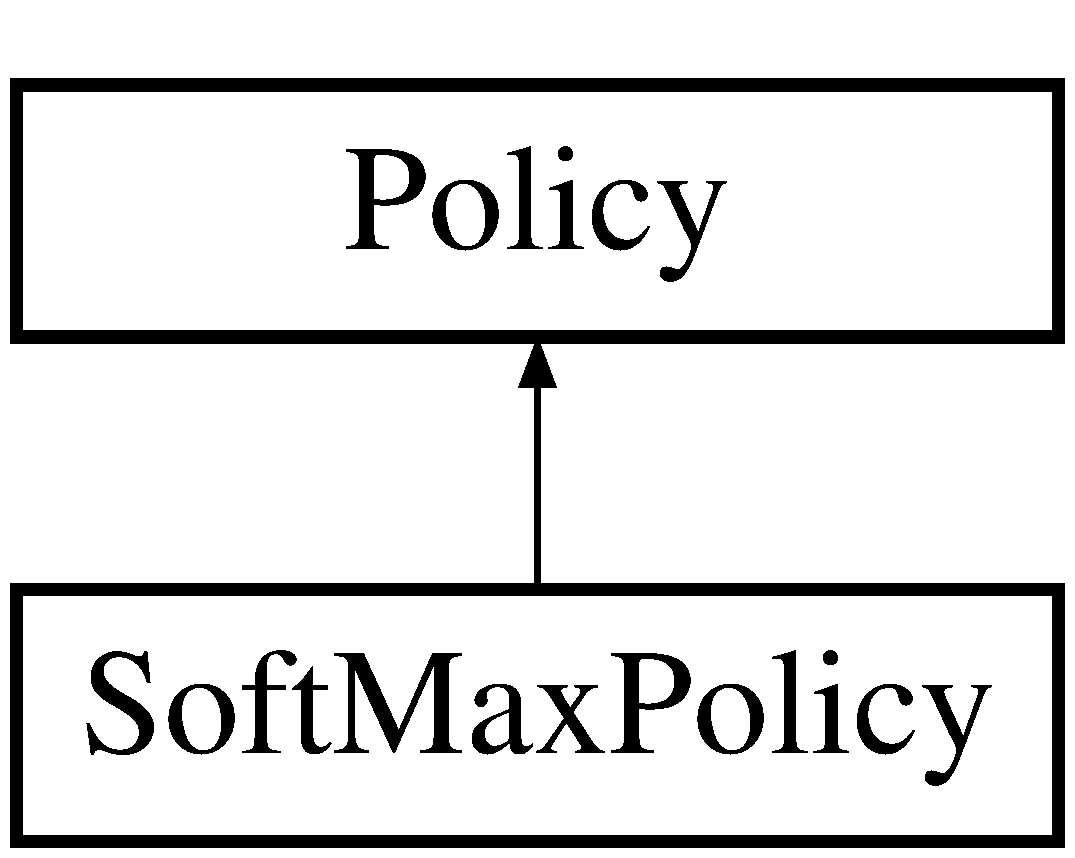
\includegraphics[height=2.000000cm]{class_soft_max_policy}
\end{center}
\end{figure}
\subsection*{Public Member Functions}
\begin{DoxyCompactItemize}
\item 
\mbox{\hyperlink{class_soft_max_policy_a9afd80b240005fc750fce1834265f80e}{Soft\+Max\+Policy}} ()=default
\item 
int \mbox{\hyperlink{class_soft_max_policy_a425d8bb5f2f504f2d7de8576f0e3f81f}{choose\+Action}} (vector$<$ int $>$ possible\+Actions, vector$<$ double $>$ num\+Values)
\end{DoxyCompactItemize}


\subsection{Detailed Description}
class of Softmax policy as explained in presentation 

\subsection{Constructor \& Destructor Documentation}
\mbox{\Hypertarget{class_soft_max_policy_a9afd80b240005fc750fce1834265f80e}\label{class_soft_max_policy_a9afd80b240005fc750fce1834265f80e}} 
\index{Soft\+Max\+Policy@{Soft\+Max\+Policy}!Soft\+Max\+Policy@{Soft\+Max\+Policy}}
\index{Soft\+Max\+Policy@{Soft\+Max\+Policy}!Soft\+Max\+Policy@{Soft\+Max\+Policy}}
\subsubsection{\texorpdfstring{Soft\+Max\+Policy()}{SoftMaxPolicy()}}
{\footnotesize\ttfamily Soft\+Max\+Policy\+::\+Soft\+Max\+Policy (\begin{DoxyParamCaption}{ }\end{DoxyParamCaption})\hspace{0.3cm}{\ttfamily [default]}}

default constructor 

\subsection{Member Function Documentation}
\mbox{\Hypertarget{class_soft_max_policy_a425d8bb5f2f504f2d7de8576f0e3f81f}\label{class_soft_max_policy_a425d8bb5f2f504f2d7de8576f0e3f81f}} 
\index{Soft\+Max\+Policy@{Soft\+Max\+Policy}!choose\+Action@{choose\+Action}}
\index{choose\+Action@{choose\+Action}!Soft\+Max\+Policy@{Soft\+Max\+Policy}}
\subsubsection{\texorpdfstring{choose\+Action()}{chooseAction()}}
{\footnotesize\ttfamily int Soft\+Max\+Policy\+::choose\+Action (\begin{DoxyParamCaption}\item[{vector$<$ int $>$}]{possible\+Actions,  }\item[{vector$<$ double $>$}]{num\+Values }\end{DoxyParamCaption})\hspace{0.3cm}{\ttfamily [inline]}, {\ttfamily [virtual]}}

chooses the next action 
\begin{DoxyParams}{Parameters}
{\em possible\+Actions} & \\
\hline
{\em num\+Values} & \\
\hline
\end{DoxyParams}
\begin{DoxyReturn}{Returns}
next action 
\end{DoxyReturn}


Reimplemented from \mbox{\hyperlink{class_policy_a7afb2eee3c77b96a58d992acb4e0e1a8}{Policy}}.



The documentation for this class was generated from the following file\+:\begin{DoxyCompactItemize}
\item 
Policy.\+h\end{DoxyCompactItemize}

\hypertarget{class_threshold_policy}{}\section{Threshold\+Policy Class Reference}
\label{class_threshold_policy}\index{Threshold\+Policy@{Threshold\+Policy}}


{\ttfamily \#include $<$Policy.\+h$>$}

Inheritance diagram for Threshold\+Policy\+:\begin{figure}[H]
\begin{center}
\leavevmode
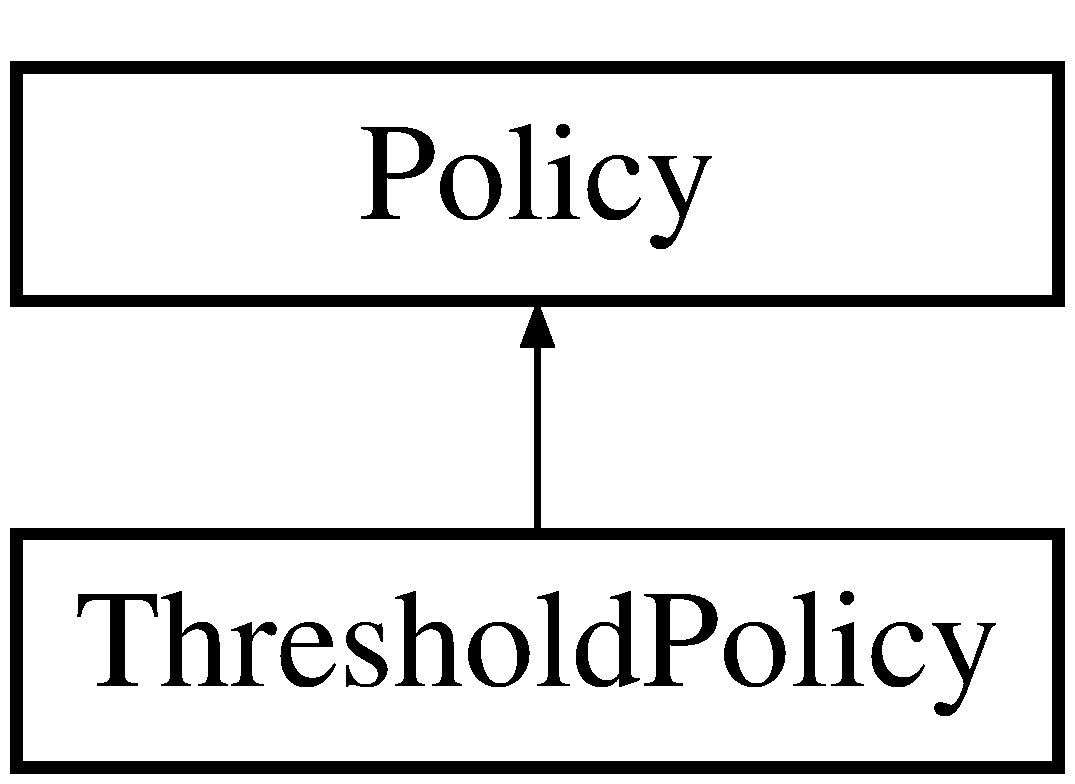
\includegraphics[height=2.000000cm]{class_threshold_policy}
\end{center}
\end{figure}
\subsection*{Public Member Functions}
\begin{DoxyCompactItemize}
\item 
pair$<$ double, int $>$ $\ast$ \mbox{\hyperlink{class_threshold_policy_aa58828f3e4165f04fb9980766ce8af06}{max\+Expected}} (vector$<$ int $>$ possible\+Actions, vector$<$ double $>$ values)
\item 
\mbox{\hyperlink{class_threshold_policy_a513adac04628872e7c7042481dc7c457}{Threshold\+Policy}} (double expl\+Rate)
\item 
int \mbox{\hyperlink{class_threshold_policy_a9f8e4051589b915971ffc647ba7fe623}{choose\+Action}} (vector$<$ int $>$ possible\+Actions, vector$<$ double $>$ num\+Values)
\end{DoxyCompactItemize}


\subsection{Detailed Description}
class of Threshold (greedy) policy as explained in presentation 

\subsection{Constructor \& Destructor Documentation}
\mbox{\Hypertarget{class_threshold_policy_a513adac04628872e7c7042481dc7c457}\label{class_threshold_policy_a513adac04628872e7c7042481dc7c457}} 
\index{Threshold\+Policy@{Threshold\+Policy}!Threshold\+Policy@{Threshold\+Policy}}
\index{Threshold\+Policy@{Threshold\+Policy}!Threshold\+Policy@{Threshold\+Policy}}
\subsubsection{\texorpdfstring{Threshold\+Policy()}{ThresholdPolicy()}}
{\footnotesize\ttfamily Threshold\+Policy\+::\+Threshold\+Policy (\begin{DoxyParamCaption}\item[{double}]{expl\+Rate }\end{DoxyParamCaption})\hspace{0.3cm}{\ttfamily [inline]}}

constructor 
\begin{DoxyParams}{Parameters}
{\em expl\+Rate} & \\
\hline
\end{DoxyParams}


\subsection{Member Function Documentation}
\mbox{\Hypertarget{class_threshold_policy_a9f8e4051589b915971ffc647ba7fe623}\label{class_threshold_policy_a9f8e4051589b915971ffc647ba7fe623}} 
\index{Threshold\+Policy@{Threshold\+Policy}!choose\+Action@{choose\+Action}}
\index{choose\+Action@{choose\+Action}!Threshold\+Policy@{Threshold\+Policy}}
\subsubsection{\texorpdfstring{choose\+Action()}{chooseAction()}}
{\footnotesize\ttfamily int Threshold\+Policy\+::choose\+Action (\begin{DoxyParamCaption}\item[{vector$<$ int $>$}]{possible\+Actions,  }\item[{vector$<$ double $>$}]{num\+Values }\end{DoxyParamCaption})\hspace{0.3cm}{\ttfamily [inline]}, {\ttfamily [virtual]}}

chooses the next action 
\begin{DoxyParams}{Parameters}
{\em possible\+Actions} & \\
\hline
{\em num\+Values} & \\
\hline
\end{DoxyParams}
\begin{DoxyReturn}{Returns}
next action 
\end{DoxyReturn}


Reimplemented from \mbox{\hyperlink{class_policy_a7afb2eee3c77b96a58d992acb4e0e1a8}{Policy}}.

\mbox{\Hypertarget{class_threshold_policy_aa58828f3e4165f04fb9980766ce8af06}\label{class_threshold_policy_aa58828f3e4165f04fb9980766ce8af06}} 
\index{Threshold\+Policy@{Threshold\+Policy}!max\+Expected@{max\+Expected}}
\index{max\+Expected@{max\+Expected}!Threshold\+Policy@{Threshold\+Policy}}
\subsubsection{\texorpdfstring{max\+Expected()}{maxExpected()}}
{\footnotesize\ttfamily pair$<$double, int$>$$\ast$ Threshold\+Policy\+::max\+Expected (\begin{DoxyParamCaption}\item[{vector$<$ int $>$}]{possible\+Actions,  }\item[{vector$<$ double $>$}]{values }\end{DoxyParamCaption})\hspace{0.3cm}{\ttfamily [inline]}}

gives back the maximal expected reward from a state given in a response 
\begin{DoxyParams}{Parameters}
{\em response} & position \\
\hline
\end{DoxyParams}
\begin{DoxyReturn}{Returns}
pair of maximal reward and its necessary action 
\end{DoxyReturn}


The documentation for this class was generated from the following file\+:\begin{DoxyCompactItemize}
\item 
Policy.\+h\end{DoxyCompactItemize}

\hypertarget{class_value_agent}{}\section{Value\+Agent Class Reference}
\label{class_value_agent}\index{Value\+Agent@{Value\+Agent}}
Inheritance diagram for Value\+Agent\+:\begin{figure}[H]
\begin{center}
\leavevmode
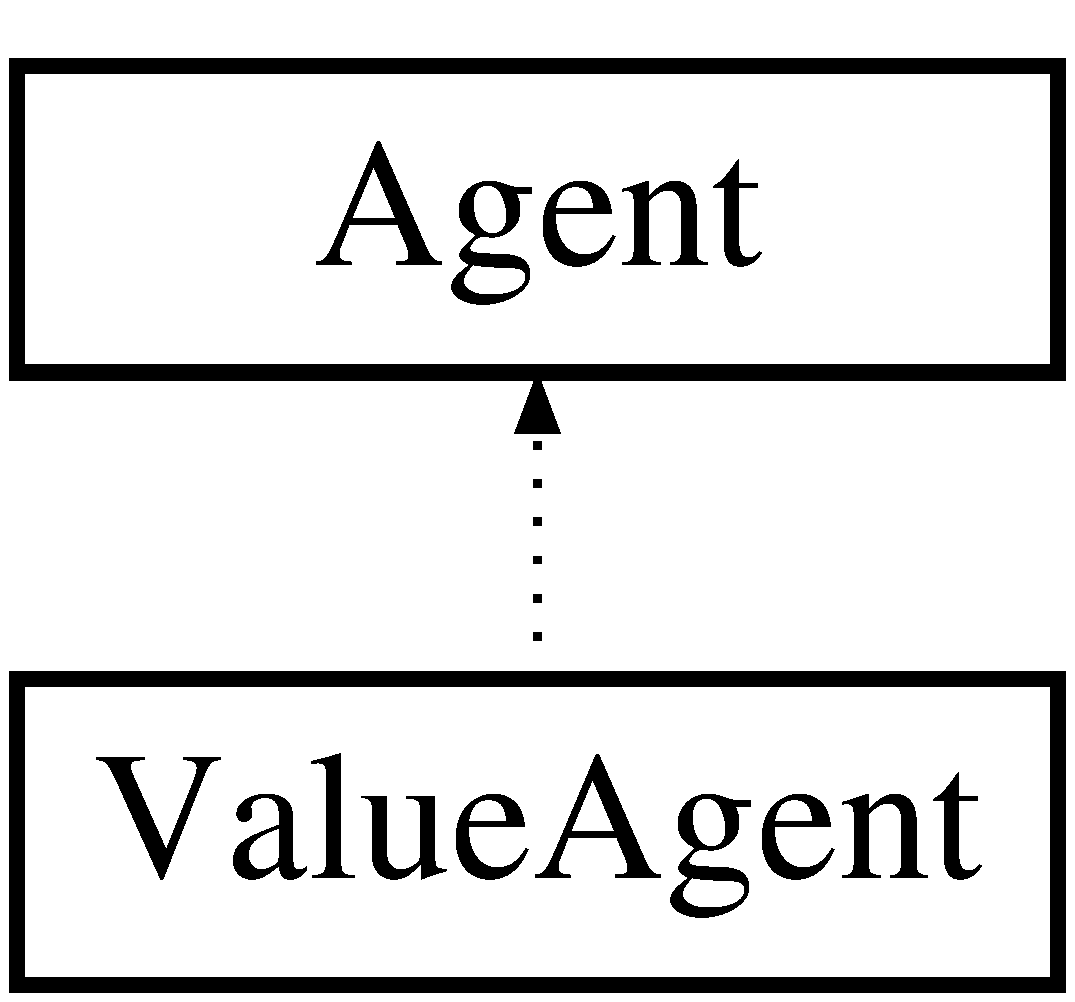
\includegraphics[height=2.000000cm]{class_value_agent}
\end{center}
\end{figure}
\subsection*{Public Member Functions}
\begin{DoxyCompactItemize}
\item 
\mbox{\Hypertarget{class_value_agent_ac1e6c8a5fba492df7323306bb69cc0f9}\label{class_value_agent_ac1e6c8a5fba492df7323306bb69cc0f9}} 
{\bfseries Value\+Agent} (double learning\+Rate, double discount\+Rate, \mbox{\hyperlink{class_policy}{Policy}} $\ast$policy, \mbox{\hyperlink{class_environment}{Environment}} $\ast$env)
\end{DoxyCompactItemize}


The documentation for this class was generated from the following file\+:\begin{DoxyCompactItemize}
\item 
Agent.\+h\end{DoxyCompactItemize}

%--- End generated contents ---

% Index
\backmatter
\newpage
\phantomsection
\clearemptydoublepage
\addcontentsline{toc}{chapter}{Index}
\printindex

\end{document}
